%%%%%%%%%%%%%%%%%%%%%%%%%%%%%%%%%%%%%%%%%%%%%%%%%%%%%%%%%%%%%%%%%%%
%TO AVOID FORMATTING ISSUES, COMPILE THIS ONLY AT WWW.OVERLEAF.COM%
%%%%%%%%%%%%%%%%%%%%%%%%%%%%%%%%%%%%%%%%%%%%%%%%%%%%%%%%%%%%%%%%%%%
%AUTHOR: ABHINAV BAKSHI
%CLASS:  BE C 302
%%%%%%%%%%%%%%%%%%%%%%%%%%%%%%%%%%%%%%%%%%%%%%%%%%%%%%%%%%%%%%%%%%%
\documentclass[a4paper,12pt]{article}
\usepackage{graphicx}
\usepackage{geometry}
\usepackage{listings}

\geometry{
	a4paper,
	total={210mm,297mm},
	left=20mm,
	right=20mm,
	top=20mm,
	bottom=20mm,
}

%To use this font, you need XeTex or LuaTex, prefer openleaf
\newenvironment{codefont}{\fontfamily{ccr}\selectfont}{\par}

\title{
	\normalfont \normalsize 
	\textsc{Pimpri Chinchwad College of Engineering \\ 
		Computer Laboratory - III} \\
	[10pt] 
	\rule{\linewidth}{0.5pt} \\[6pt] 
	\huge Assignment No - A6 \\
	\rule{\linewidth}{2pt}  \\[10pt]
}
\author{}
\date{\normalsize}


\begin{document}
	\maketitle
	
\section{TITLE : }   Select an Industrial sector and write an application using BIA tool for maximizing the profit.

\begin{itemize}
	\item Design an application using tool for clustering the iris flowers dataset.
	\item Design an application using tool to predict whether to play tennis or not.
	
\end{itemize}

\section{MATHEMATICAL MODEL : }

{\rmfamily
	Mathematical model is given as below,}


\bigskip

\textrm{\textbf{S=fs,e,X,Y,Fme,DD,NDD,Mem\_shared}}


\bigskip

{\rmfamily
	Where,}

{\rmfamily
	\textbf{s = Initial State}}

{\rmfamily
	\textbf{e = End State}}

{\rmfamily
	\textbf{X=Input}\\
	Datasets of iris flowers and tennis.
	}
	
	{\rmfamily
		\textbf{Y=Osutput}\\
		Clustering of iris flowers and prediction whether to play tennis or not, \\using the interactive table, scatterplot, histogram, etc.}
	
	{\rmfamily
		\textbf{Fme=Algorithms used (K-means and Naïve-Bayes)}
		
		
			\begin{itemize}
				\item K-means Algorithm : (Used for iris dataset)
				
				\begin{enumerate}
					\item Randomly select ‘c’ cluster centers.
					\item Calculate the distance between each data point and cluster centers.
					\item  Assign the data point to the cluster center whose distance from the cluster center is minimum of all the cluster centers..
					\item  Recalculate the new cluster center using:  
					\begin{center}
						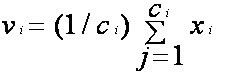
\includegraphics[scale=0.5]{equation.jpg}
					\end{center}
					where, ‘ci’ represents the number of data points in ith cluster.
					\item Recalculate the distance between each data point and new obtained cluster centres.
					\item If no data point was reassigned then stop, otherwise repeat from step 3.
					
				\end{enumerate}
				
				\item Naïve-Bayes Algorithm : (Used for tennis dataset)
				
				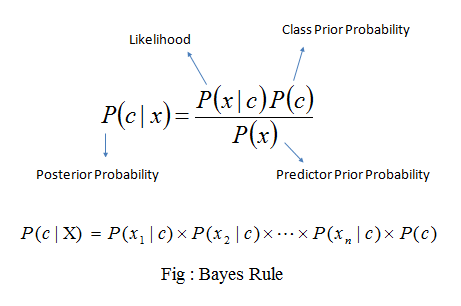
\includegraphics[scale=0.5]{nb.png}
			\end{itemize}
			
			\newpage
			\textbf{K-means example : }
			
			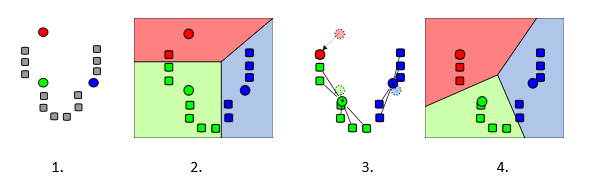
\includegraphics{kmeanseg.png}
	
			\begin{enumerate}
				\item	k initial "means" (in this case k=3) are randomly generated within the data domain (shown in color)
				\item	k clusters are created by associating every observation with the nearest mean. The partitions here represent the diagram generated by the means 
				\item	The centroid of each of the k clusters becomes the new mean.
				\item	Steps 2 and 3 are repeated until convergence has been reached.
				
			\end{enumerate}
			
			\textbf{Naive-Bayes Example : }
			\begin{center}
				\begin{figure}[!htbp]
					\centering
					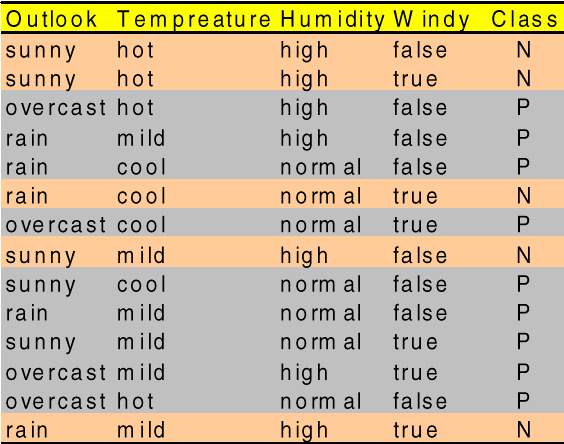
\includegraphics{nb1.png}
					\caption{Given a training set, we can compute the probabilities}
				\end{figure}
			\end{center} 
			\newpage
				\begin{center}
					\begin{figure}[!htbp]
						\centering
						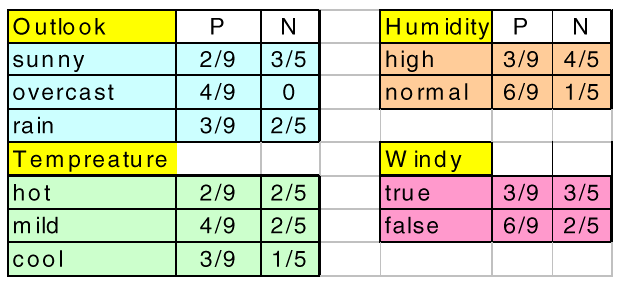
\includegraphics{nb2.png}
					\end{figure}
				\end{center}
			

			$X = <sunny, mild, high, true>$
			\\
			$Pr(X | “no”).Pr(“no”) = (3/5 . 2/5 . 4/5 . 3/5) . 5/14 = 0.04$
			\\
			$Pr(X | “yes”).Pr(“yes”) = (2/9 . 4/9 . 3/9 . 3/9) . 9/14 = 0.007$
			\\
		
		
		
		
		
		
		
		
		
		
		
		
		
		
		
		
		
		
		
		}
	
	{\rmfamily
		\textbf{DD=Deterministic Data}\\
		Iris dataset,Tennis Dataset.
	}
	
	{\rmfamily
		\textbf{NDD=Non -Deterministic Data}\\
		Number of clusters, etc.}
	
	{\rmfamily
		\textbf{Mem-shared}=memory shared by the applications.}
	
	
	\bigskip

\section{THEORY : }

\subsection{Introduction to Business Analytics and Intelligence :}

\textbf{Business Analytics :}\\
Business analytics (BA) is the practice of iterative, methodical exploration of an organization's data with emphasis on statistical analysis.\\ Business analytics is used by companies committed to data-driven decision making.


Business Intelligence is querying, reporting, OLAP, and alert tools can answer questions such as what happened, how many, how often, where the problem is, and what actions are needed. Business analytics can answer questions like why is this happening, what if these trends continue, what will happen next (that is, predict), what is the best that can happen (that is, optimize).\\

Some examples of BA are :

\begin{itemize}
	\item Exploring data to find new patterns and relationships (data mining)
	\item Forecasting future results (predictive modeling, predictive analytics)
	\item Explaining why a certain result occurred (statistical analysis, quantitative analysis)
\end{itemize}
	

\textbf{Business Intelligence :}\\
\\
Business intelligence (BI) is often described as "the set of techniques and tools for the transformation of raw data into meaningful and useful information for business analysis purposes".  

BI technologies are capable of handling large amounts of unstructured data to help identify, develop and otherwise create new strategic business opportunities. The goal of BI is to allow for the easy interpretation of these large volumes of data. Identifying new opportunities and implementing an effective strategy based on insights can provide businesses with a competitive market advantage and long-term stability. 

BI technologies provide historical, current and predictive views of business operations. Common functions of business intelligence technologies are  reporting, online analytical processing, analytics, data mining, process mining, complex event processing, business performance management, benchmarking, text mining, predictive analytics and prescriptive analytics.

BI can be used to support a wide range of business decisions ranging from operational to strategic.


\textbf{KNIME tool :}\\
\\
KNIME, the Konstanz Information Miner, is an open source data analytics, reporting and integration platform. KNIME integrates various components for machine learning and data mining through its modular data pipelining concept. A graphical user interface allows assembly of nodes for data pre-processing \(ETL: Extraction, Transformation, Loading\), for modelling and data analysis and visualization.
Since 2006, KNIME has been used in pharmaceutical research,[2] but is also used in other areas like CRM customer data analysis, business intelligence and financial data analysis.


Innovative organizations use our open-source, enterprise-grade analytics platform to discover the potential hidden in their data, mine for fresh insights or predict new futures. It is quick to deploy, easy to scale, and intuitive, KNIME is used in over 60 countries on data of every kind: from numbers to images, molecules to humans, signals to complex networks, from kilo- to petabytes, or simple reports to complex analyses.

\section{Conclusion : }

Hence, we have designed an application using tool for categorizing the iris flowers dataset and an application to predict whether to play tennis or not.

\section{References}

\begin{enumerate}
	\item 	“Data Mining Concepts and Techniques”,Second Edition,Jiawei Han,Micheline Kamber,Jian Pei.
	\item	https://www.knime.org/knime
	\item	http://searchdatamanagement.techtarget.com/definition/business-intelligence
	\item	http://www.webopedia.com/TERM/B/Business\_Intelligence.html
	\item	http://searchbusinessanalytics.techtarget.com/definition/business-analytics-BA	
\end{enumerate}


\newpage
	\begin{itemize} 	

\item Input:

Training and Input Data:
 \begin{center}
	\begin{figure}[!htbp]
		\centering
		\fbox{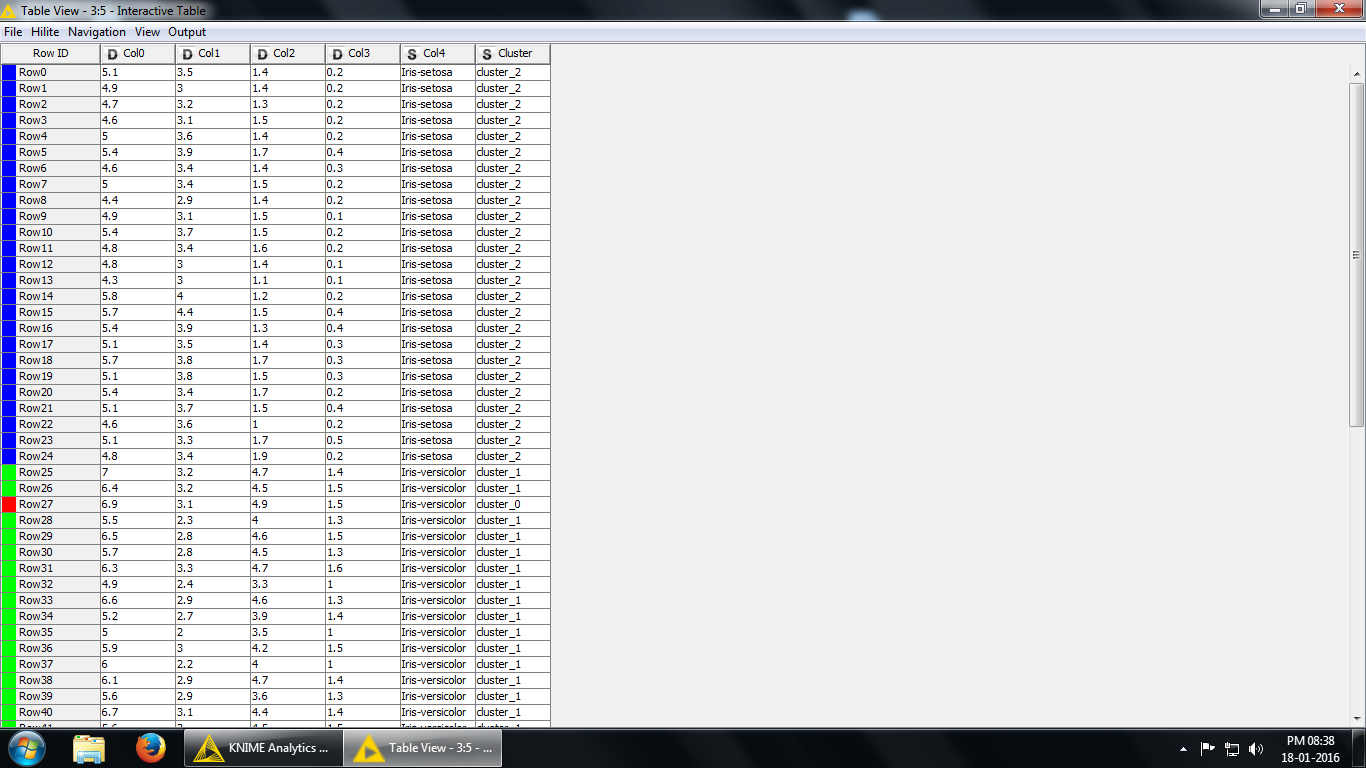
\includegraphics[scale=0.30]{input-interactive table1 kmeans.png}}	
	\end{figure}
\end{center} 

\begin{center}
	\begin{figure}[!htbp]
		\centering
		\fbox{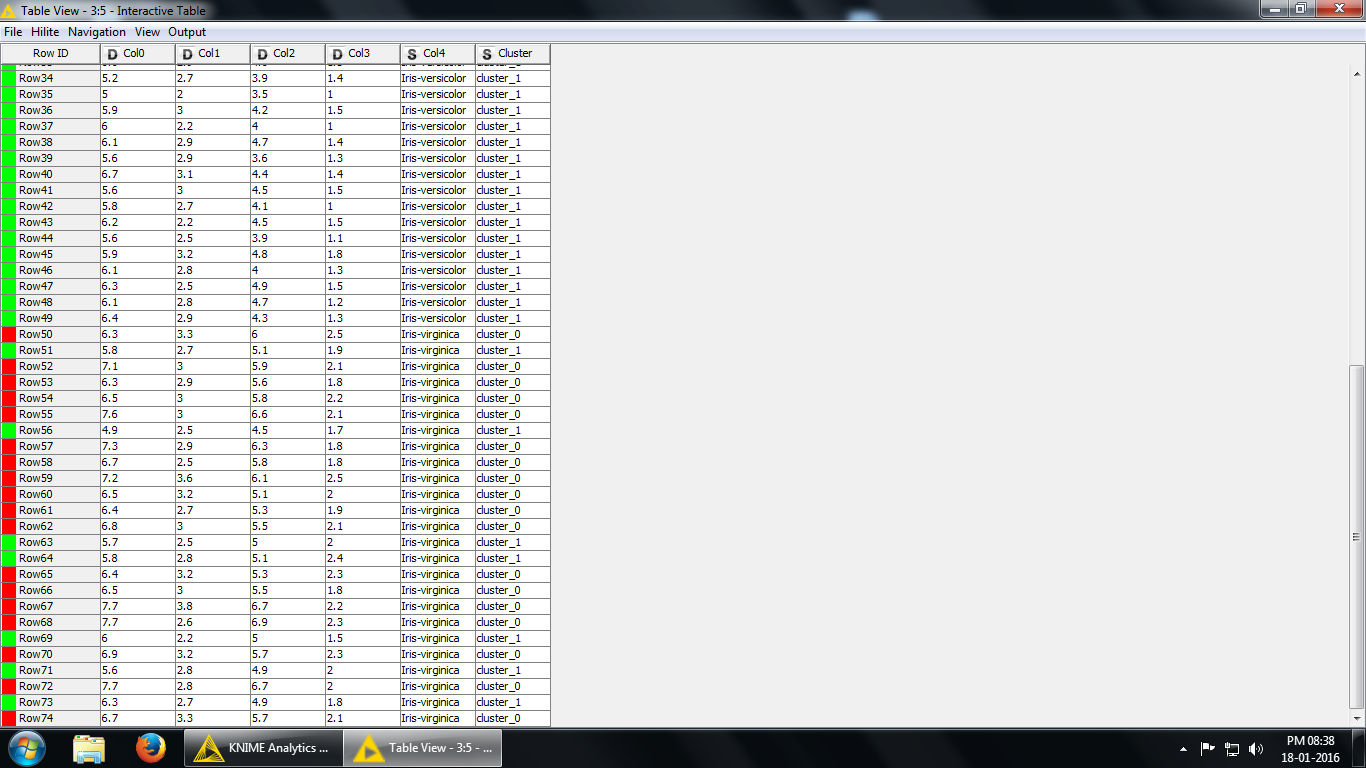
\includegraphics[scale=0.30]{input-interactive table2 kmeans.png}}	
	\end{figure}
\end{center} 

\newpage
\item Knime Design:

Training and Input Data:
\begin{center}
	\begin{figure}[!htbp]
		\centering
		\fbox{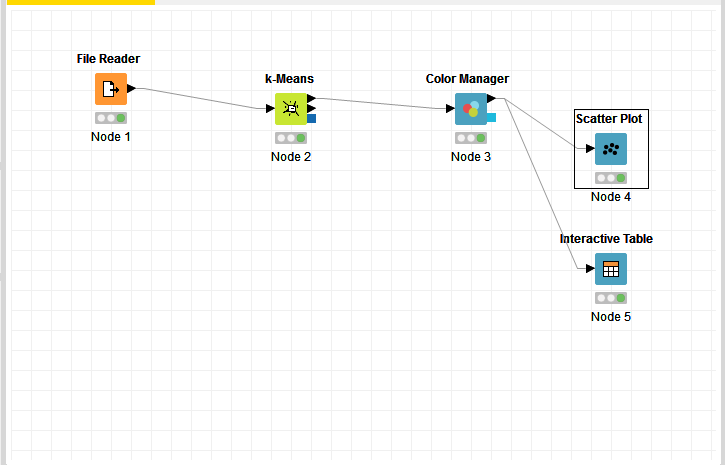
\includegraphics[scale=0.50]{k-means.png}}	
	\end{figure}
\end{center} 

\begin{center}
	\begin{figure}[!htbp]
		\centering
		\fbox{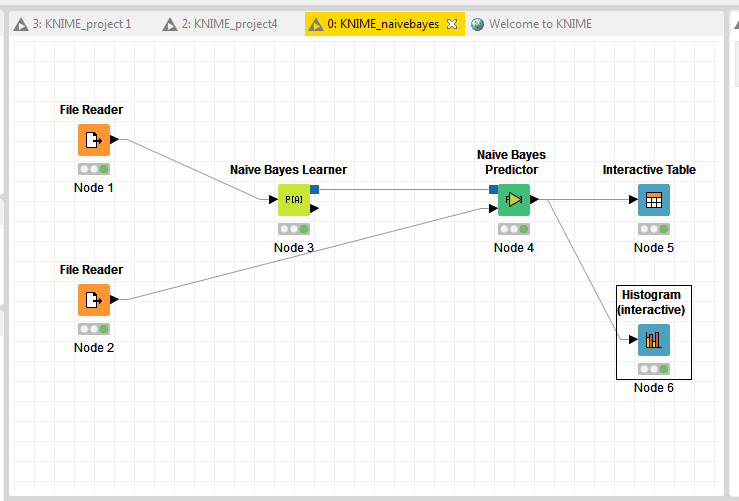
\includegraphics[scale=0.50]{naive_bayes.png}}	
	\end{figure}
\end{center} 
\newpage

\item Output

\begin{center}
	\begin{figure}[!htbp]
		\centering
		\fbox{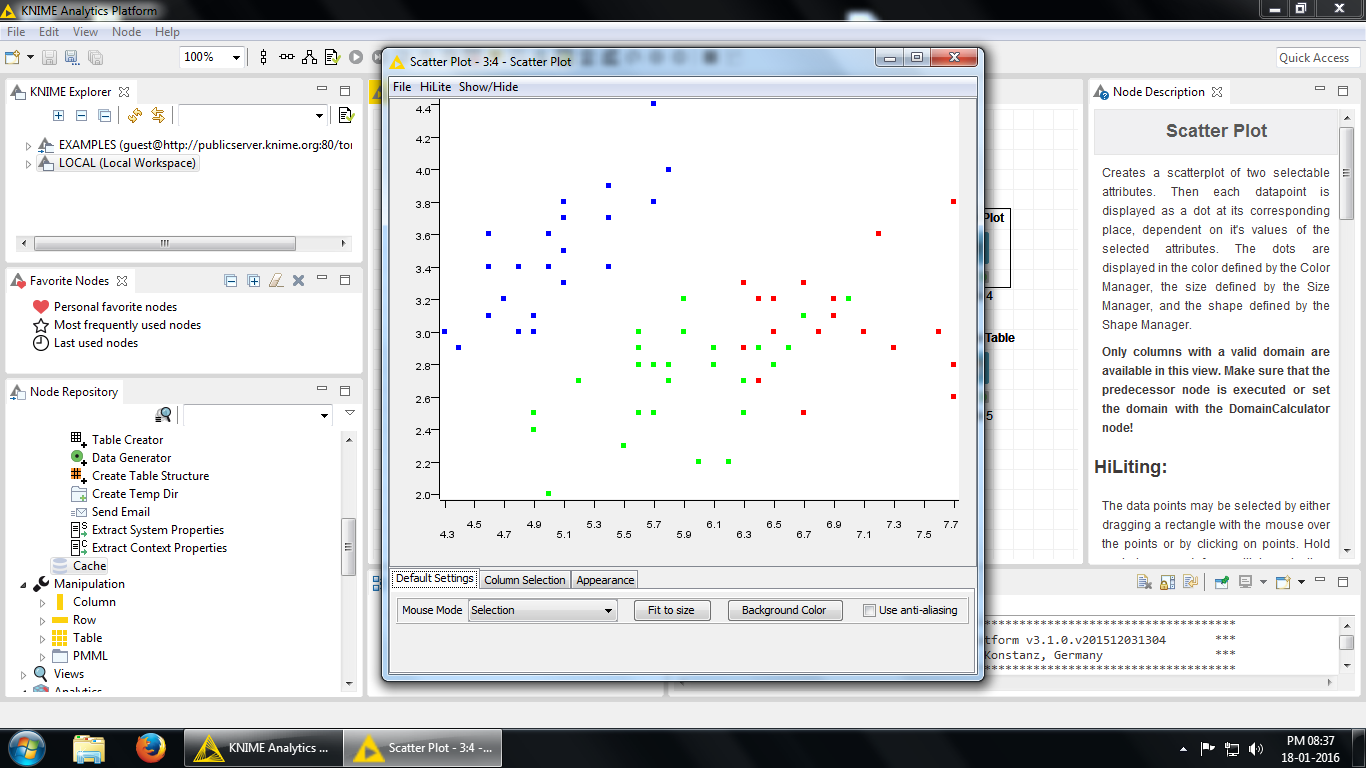
\includegraphics[scale=0.30]{output-scatter plot k-means.png}}	
	\end{figure}
\end{center} 

\begin{center}
	\begin{figure}[!htbp]
		\centering
		\fbox{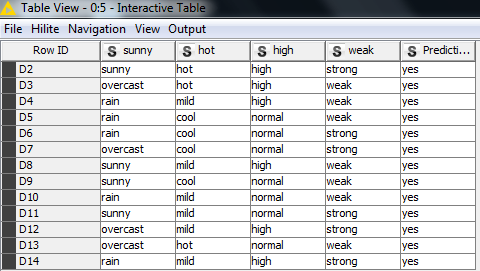
\includegraphics{output-N_B.png}}	
	\end{figure}
\end{center} 
\begin{center}
	\begin{figure}[!htbp]
		\centering
		\fbox{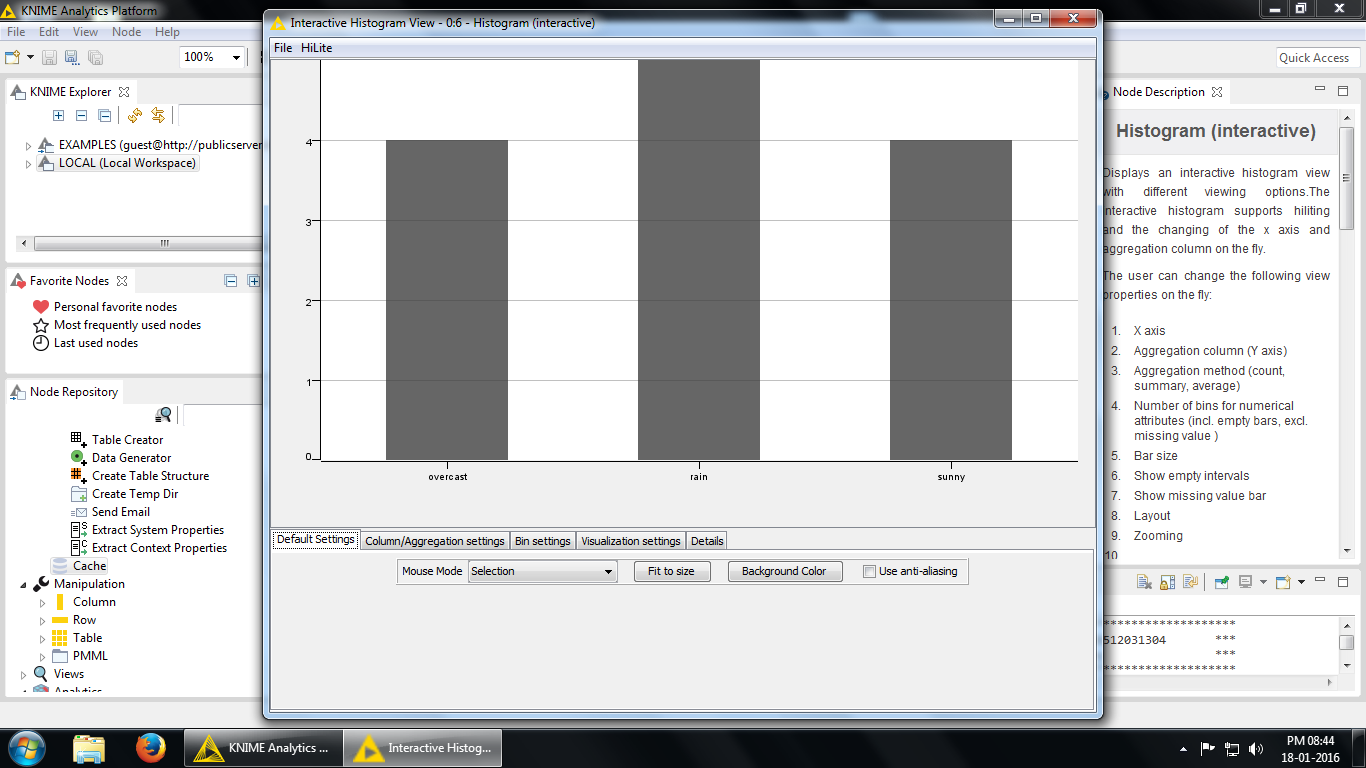
\includegraphics[scale=0.50]{output-N-B_histogram.png}}	
	\end{figure}
\end{center} 
\end{itemize}
\begin{center}
\newpage	
	\begin{tabular}
		{|c|c|c|c|c|}\hline
		{\bf Roll No.}		&{\bf Name of Student}	&{\bf Date of Performance}  				&{\bf Date of Submission}	&{\bf Sign.}  \\    \hline
		302	& Abhinav Bakshi & 15/12/2015	& 	5/01/2016	&  \\ \hline
	\end{tabular}\\ 
\end{center}	

\end{document}
}